\documentclass[a4paper,10pt]{article}
\usepackage[utf8]{inputenc}
\usepackage[spanish]{babel}
\usepackage{fancyhdr}
\usepackage{multicol}
\usepackage{geometry}
\usepackage{amsmath}
\usepackage{fancybox}
\usepackage{graphicx}

\geometry{a4paper, portrait, margin=1in}

\pagestyle{fancy}
\fancyhf{}
\fancyhead[L]{\textbf{Estadística Computacional}}
\fancyhead[R]{Universidad Nacional del Altiplano - FINESI}
\fancyfoot[C]{\thepage}

\begin{document}

\section*{Evaluación – Métodos de Optimización \\{Docente: Torres Cruz Fred } \\ \large 28 de mayo de 2025} \

\vspace{0.5cm}
\textbf{Apellidos y Nombres:  Ccora Quispe Kenny Leonel }  \hfill \textbf{Código:231985} 

\vspace{0.5cm}
\section*{1. Evaluación Teórica}

\begin{enumerate}
    \item ¿Cuál de las siguientes afirmaciones describe mejor una función lineal?
    \begin{itemize}
        \item a) Es una función que tiene exponentes no lineales
        \item b) Es una función que se representa gráficamente como una curva
        \item \fbox{c) Es una función cuya gráfica es una línea recta}
        \item d) Es una función que involucra productos de variables
        \item e) Es una función con términos cuadráticos
    \end{itemize}

    \item En programación lineal, ¿cuál es el principal objetivo de las restricciones?
    \begin{itemize}
        \item a) Minimizar el número de variables en la función objetivo
        \item \fbox{b) Establecer las condiciones bajo las cuales se deben encontrar soluciones}
        \item c) Maximizar el valor de la función objetivo
        \item d) Aumentar el número de soluciones posibles
        \item e) Simplificar el cálculo de la función objetivo
    \end{itemize}

    \item ¿Qué concepto define el conjunto de todas las soluciones posibles que satisfacen las restricciones de un problema de optimización?
    \begin{itemize}
        \item \fbox{a) Región factible}
        \item b) Función objetivo
        \item c) Solución degenerada
        \item d) Solución óptima
        \item e) Solución no acotada
    \end{itemize}

    \item ¿Cuál de los siguientes es un objetivo típico en los problemas de optimización?
    \begin{itemize}
        \item a) Hallar el máximo local de una función
        \item \fbox{b) Encontrar el valor mínimo o máximo de una función objetivo sujeta a restricciones}
        \item c) Minimizar el número de variables
        \item d) Encontrar soluciones inexactas para ecuaciones no lineales
        \item e) Resolver integrales definidas
    \end{itemize}

    \item ¿Qué condición debe cumplirse para que un sistema de ecuaciones lineales tenga una única solución?
    \begin{itemize}
        \item a) El determinante de la matriz asociada debe ser cero
        \item b) El sistema debe ser homogéneo
        \item \fbox{c) El determinante de la matriz asociada debe ser distinto de cero}
        \item d) El sistema debe ser dependiente
        \item e) No debe haber ninguna restricción adicional
    \end{itemize}

    \item Una empresa produce sillas (\(x\)) y mesas (\(y\)). Cada silla genera una utilidad de 40 y cada mesa 60. Si la función objetivo es Maximizar \(Z = 40x + 60y\), ¿qué representa el valor 60?
    \begin{itemize}
        \item a) El costo de producir una mesa
        \item \fbox{b) La utilidad unitaria por cada mesa vendida}
        \item c) El número máximo de mesas que se pueden producir
        \item d) El tiempo necesario para producir una mesa
        \item e) El precio de venta de una mesa
    \end{itemize}

    \item ¿Qué tipo de función es típicamente la función objetivo en programación lineal?
    \begin{itemize}
        \item a) Una función cuadrática
        \item b) Una función polinómica
        \item \fbox{c) Una función lineal}
        \item d) Una función logarítmica
        \item e) Una función exponencial
    \end{itemize}

    \item ¿Qué diferencia hay entre restricciones de igualdad y restricciones de desigualdad en programación lineal?
    \begin{itemize}
        \item a) Las restricciones de igualdad no afectan el resultado
        \item \fbox{b) Las restricciones de desigualdad limitan el conjunto factible, mientras que las de igualdad lo definen completamente}
        \item c) Solo las restricciones de desigualdad son necesarias para resolver el problema
        \item d) Las restricciones de igualdad simplifican el cálculo de la función objetivo
        \item e) Las restricciones de desigualdad no limitan el espacio de soluciones
    \end{itemize}

    \item ¿Cuál de los siguientes no es un tipo de restricción en programación lineal?
    \begin{itemize}
        \item a) Restricciones de igualdad
        \item b) Restricciones de desigualdad
        \item c) Restricciones implícitas
        \item \fbox{d) Restricciones no lineales}
        \item e) Restricciones de viabilidad
    \end{itemize}

    \item En la teoría de la optimización, el tiempo de ejecución de un algoritmo depende principalmente de:
    \begin{itemize}
        \item a) El número de variables del problema
        \item b) El número de soluciones óptimas
        \item c) El tipo de función objetivo
        \item d) La cantidad de restricciones
        \item \fbox{e) La complejidad del algoritmo utilizado}
    \end{itemize}
\end{enumerate}

\newpage
\section*{2. Evaluación Práctica}

\subsection*{Pregunta 1 }

Una empresa realiza análisis de datos de redes sociales para predecir tendencias en el mercado local.  
El departamento de análisis utiliza dos tipos de servidores: Servidor A y Servidor B.  
El Servidor A puede procesar 500 GB de datos en 10 horas, mientras que el Servidor B procesa 300 GB en 8 horas.  
Ambos servidores tienen un límite máximo de funcionamiento diario de 12 horas, y el almacenamiento total disponible en la empresa es de 4000 GB por día.  
Además, el costo de energía por hora en el Servidor A es de 50 soles y en el Servidor B es de 30 soles.  
\textbf{El objetivo es maximizar la cantidad de datos procesados al día sin superar el presupuesto de 1200 soles diarios en energía.}

\vspace{0.5cm}
\textbf{Resolución (imagen):}
\begin{center}
    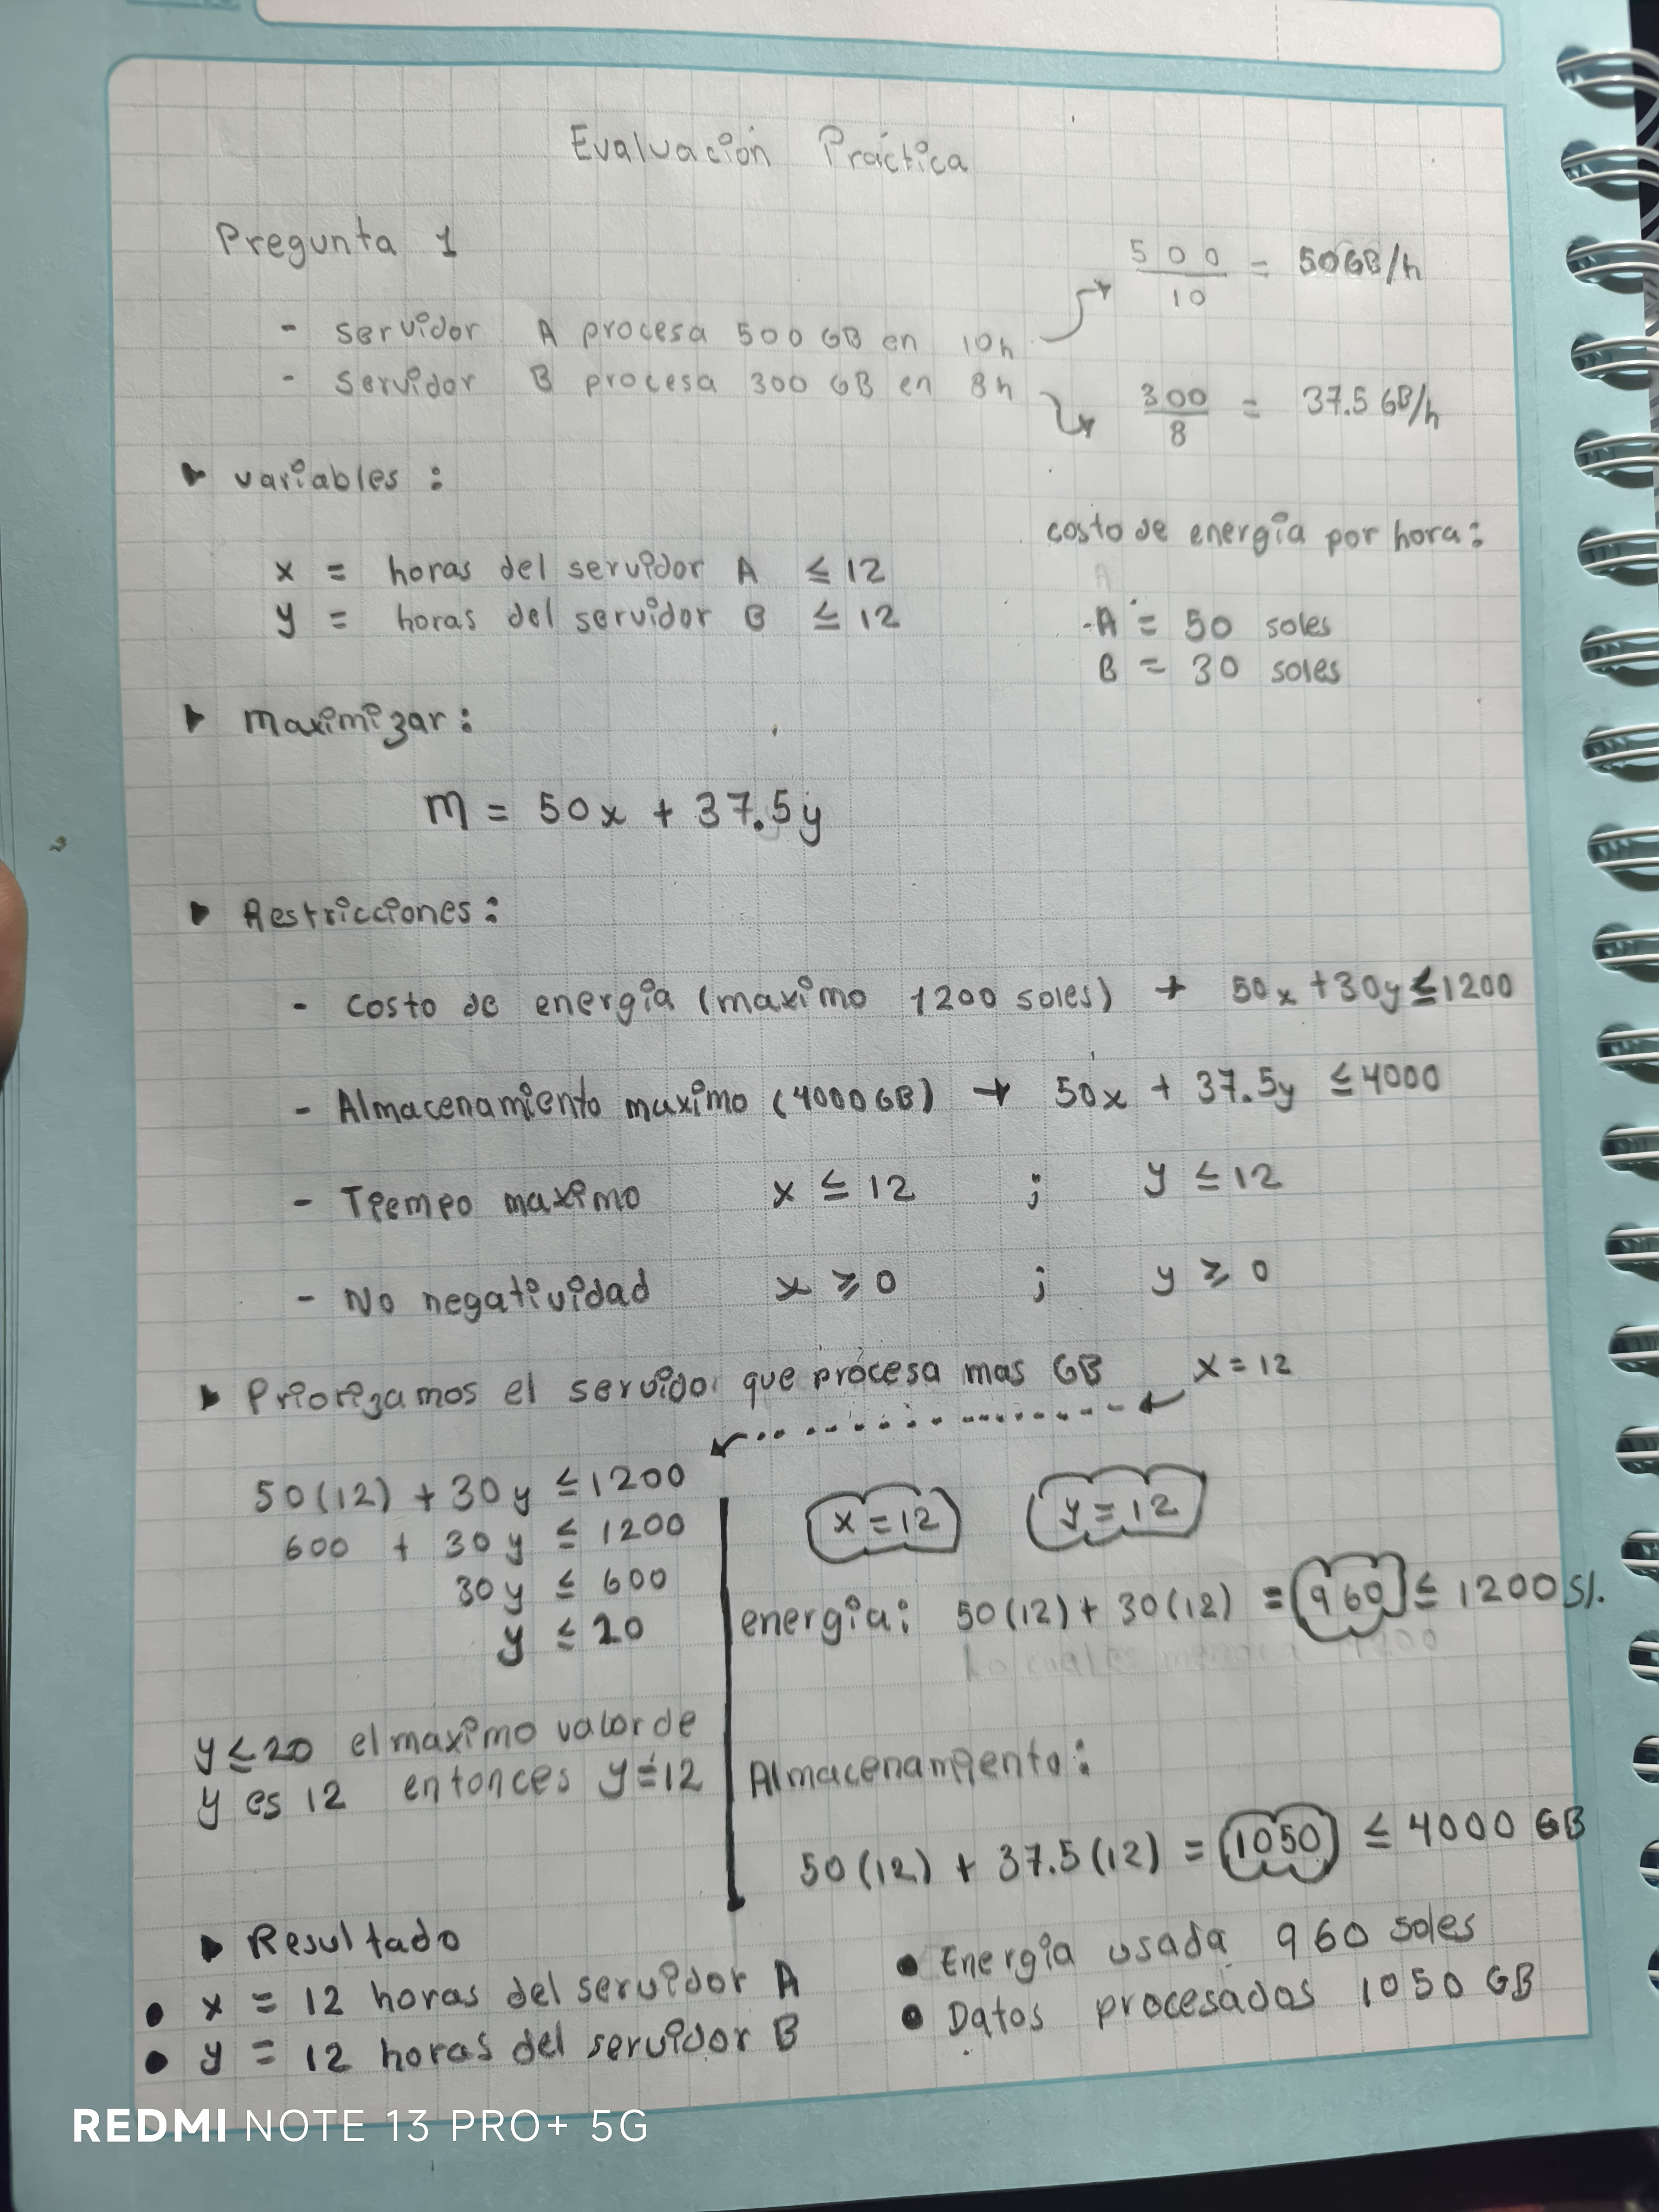
\includegraphics[width=0.95\textwidth]{pregunta1.png}
\end{center}

\vspace{1cm}
\subsection*{Pregunta 2}

Una empresa de seguridad monitorea sistemas de videovigilancia y debe analizar imágenes de alta resolución.  
Tiene dos centros de procesamiento: Centro A y Centro B.  
El Centro A puede analizar 80 imágenes por hora, y el Centro B puede analizar 100 imágenes por hora.  
Debido a los costos de mantenimiento, el Centro A no puede operar más de 10 horas al día y el Centro B no puede operar más de 12 horas al día.  
El sistema debe procesar al menos 1200 imágenes al día, y cada centro tiene un límite de almacenamiento de 600 imágenes al día.  
\textbf{El objetivo es minimizar el número de horas de operación de ambos centros, asegurando que el número mínimo de imágenes procesadas sea alcanzado.}

\vspace{0.5cm}
\textbf{Resolución (imagen):}
\begin{center}
    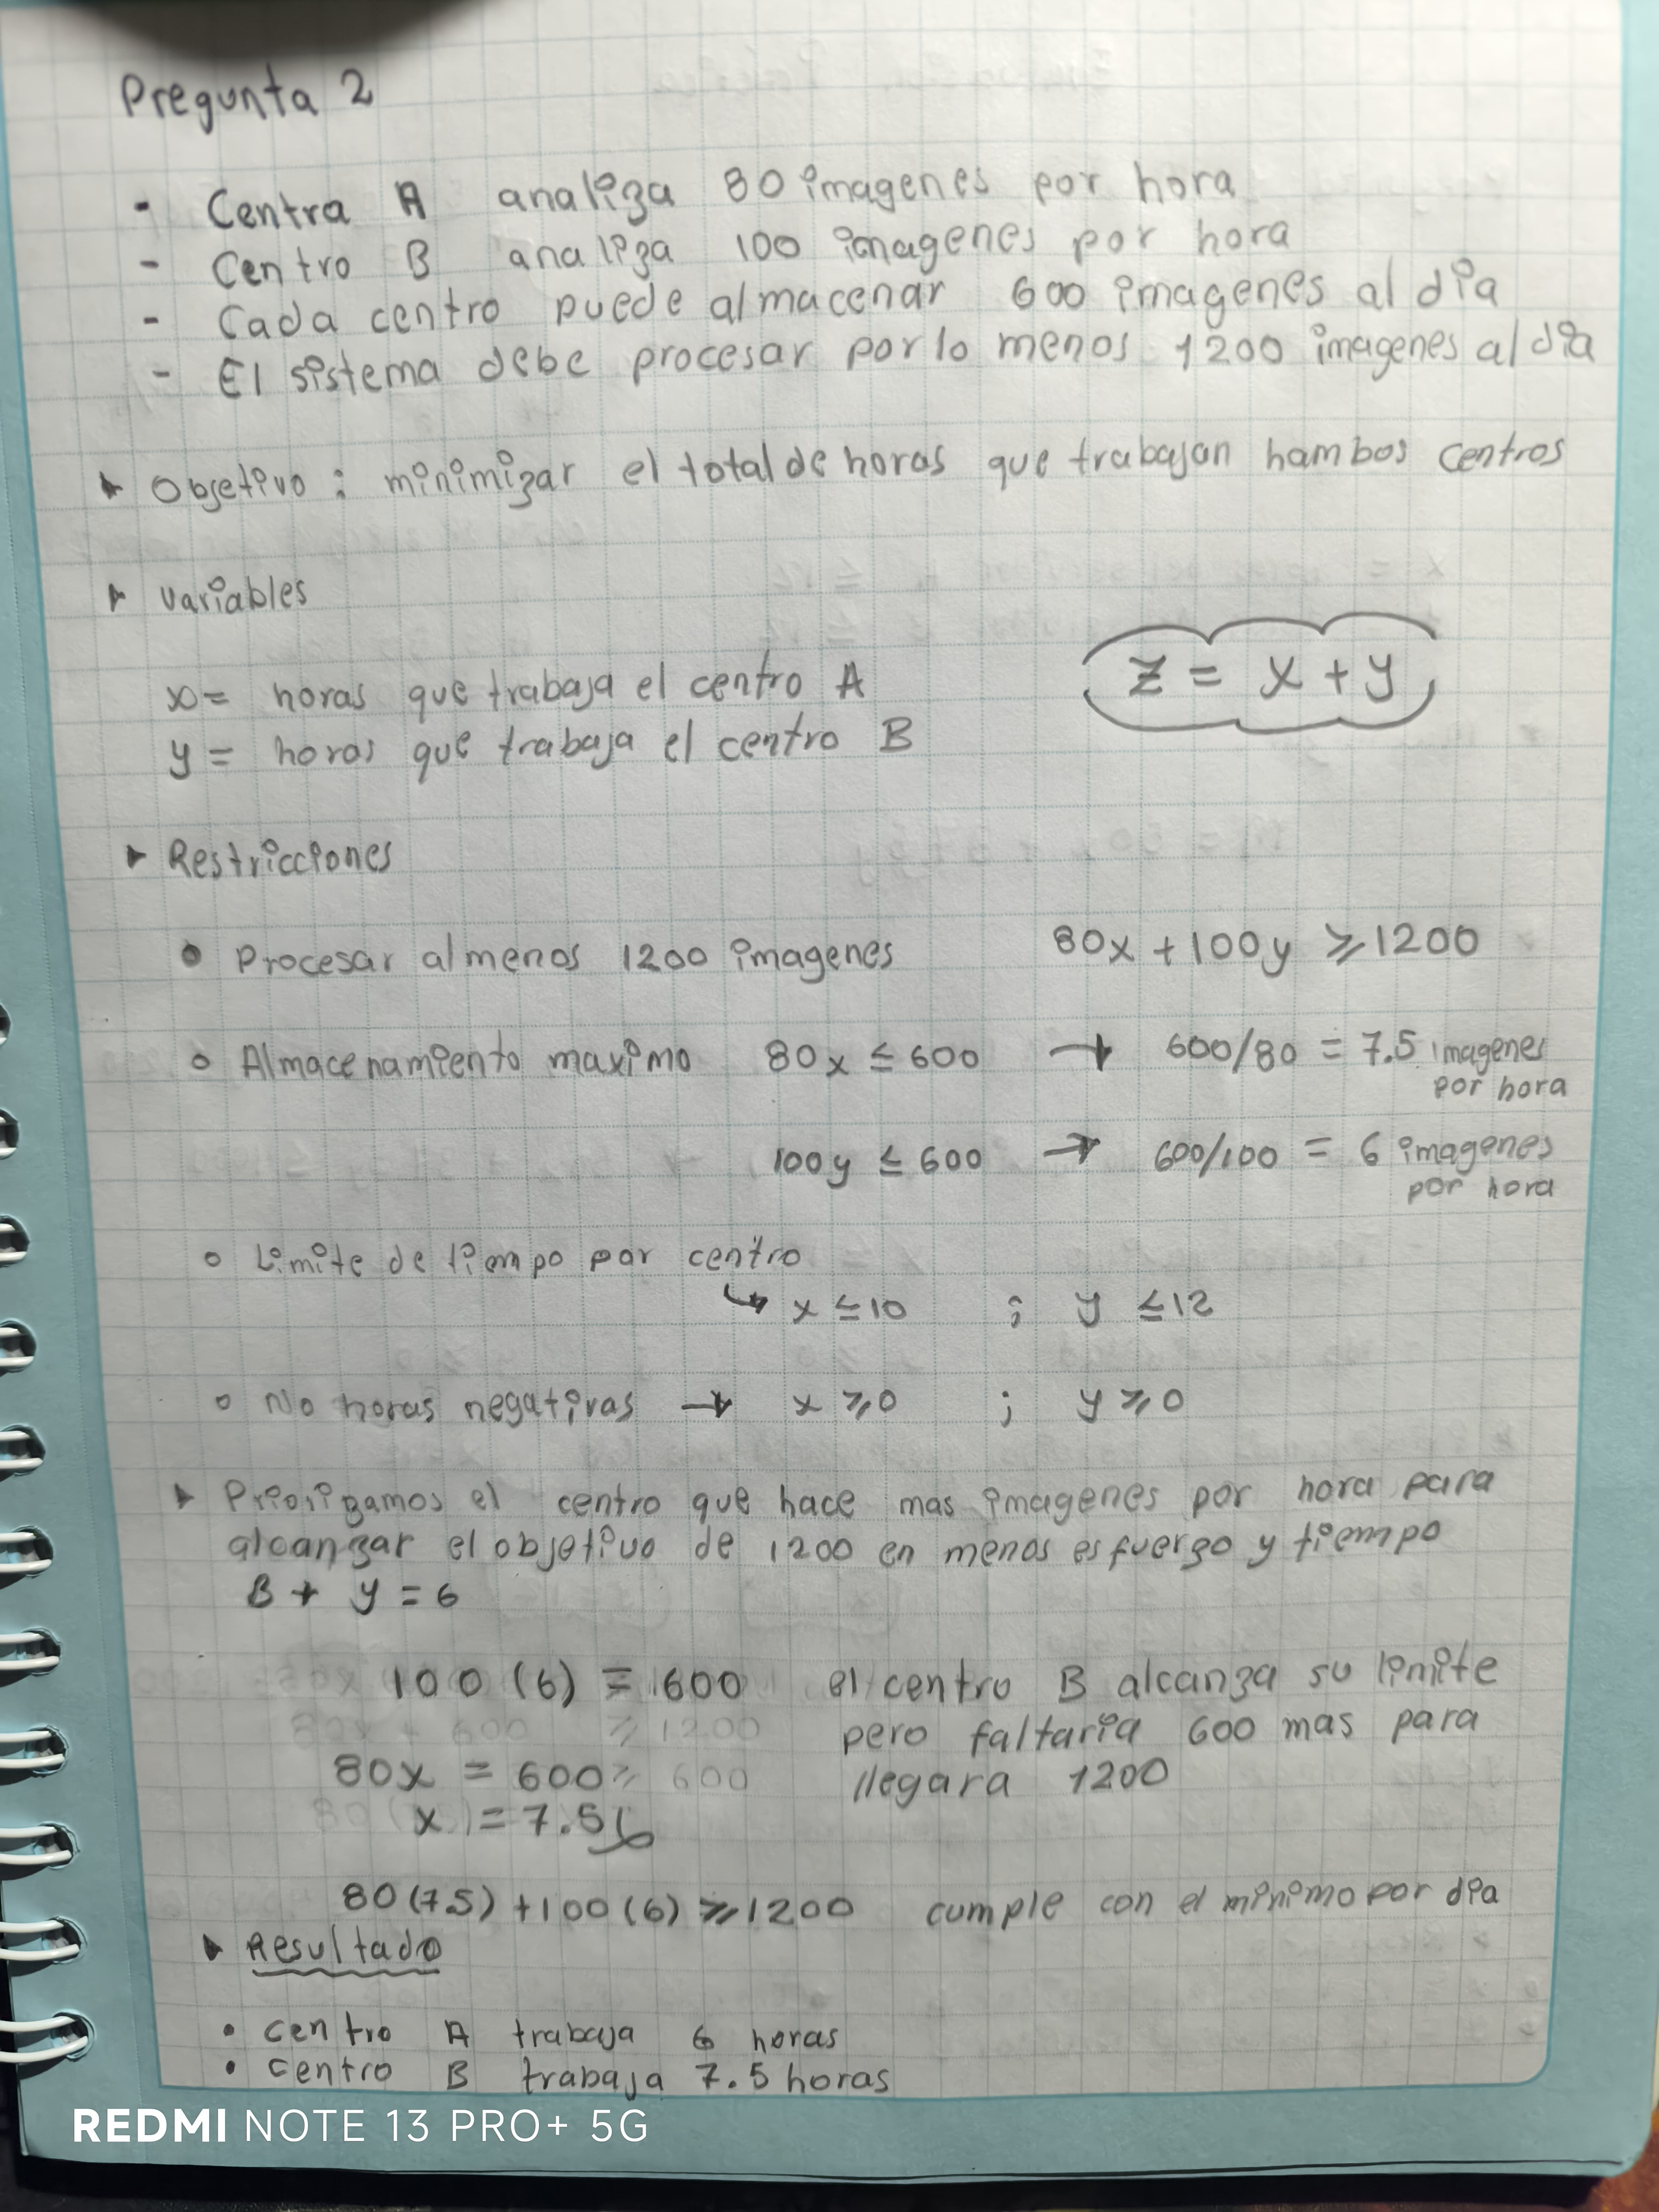
\includegraphics[width=0.95\textwidth]{pregunta2.png}
\end{center}

\end{document}
